\documentclass[letterpaper,12pt,fleqn]{article}
\usepackage{matharticle}
\usepackage{tikz}
\usetikzlibrary{arrows}
\pagestyle{empty}
\newcommand{\T}{\mathscr{T}}
\renewcommand{\a}{\alpha}
\renewcommand{\b}{\beta}
\renewcommand{\l}{\lambda}
\newcommand{\e}{\epsilon}
\begin{document}
\section*{Connectedness}

Intuitively, a topological space \(X\) exists as a single piece.

\begin{example}[Disconnected]
  \begin{minipage}{3in}
    \centering

    \bigskip

    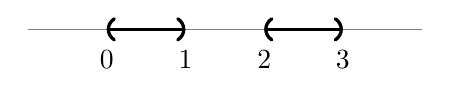
\begin{tikzpicture}
      \draw [help lines] (-1,0) -- (4,0);
      \draw [(-),very thick] (0,0) -- (1,0);
      \draw [(-),very thick] (2,0) -- (3,0);
      \node [below=1ex] at (0,0) {\(0\)};
      \node [below=1ex] at (1,0) {\(1\)};
      \node [below=1ex] at (2,0) {\(2\)};
      \node [below=1ex] at (3,0) {\(3\)};
    \end{tikzpicture}

    \bigskip

    \(X=(0,1)\cup(2,3)\)
  \end{minipage}
  \begin{minipage}{3in}
    \centering

    \bigskip

    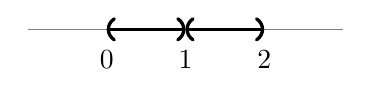
\begin{tikzpicture}
      \draw [help lines] (-1,0) -- (3,0);
      \draw [(-),very thick] (0,0) -- (1,0);
      \draw [(-),very thick] (1,0) -- (2,0);
      \node [below=1ex] at (0,0) {\(0\)};
      \node [below=1ex] at (1,0) {\(1\)};
      \node [below=1ex] at (2,0) {\(2\)};
    \end{tikzpicture}

    \bigskip

    \(X=(0,1)\cup(1,2)\)
  \end{minipage}
\end{example}

There are two notions of connectedness:
\begin{enumerate}
\item Connected: One piece
\item Path Connected: The ability to \emph{walk} from any point to any other.

  \bigskip

  \begin{tikzpicture}[dot node/.style={draw,circle,fill,inner sep=0cm,minimum size=0.1cm}]
    \draw (0,0) ellipse (4cm and 2cm);
    \node [dot node] (P) at (-2cm,-0.5cm) {};
    \node [below] at (P) {\(p\)};
    \node [dot node] (Q) at (2cm,0.5cm) {};
    \node [below] at (Q) {\(q\)};
    \draw [dashed] (P) to (Q);
  \end{tikzpicture}
\end{enumerate}

\begin{example}[The Topologists Sine Curve]
  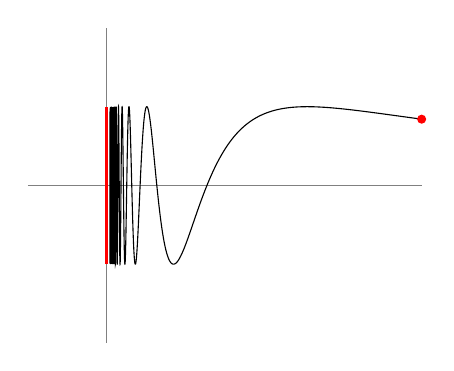
\begin{tikzpicture}
    \draw [help lines] (-1,0) -- (4,0);
    \draw [help lines] (0,-2) -- (0,2);
    \draw [samples=10000,domain=0.04:4] plot ({\x},{sin(deg(4/(\x)))});
    \draw [red,very thick] (0,-1) -- (0,1);
    \node [draw,circle,fill,red,inner sep=0cm,minimum width=0.1cm] at (4,{sin(deg(1))}) {};
  \end{tikzpicture}
  \begin{gather*}
    S=\setb{\left(x,\sin\left(\frac{1}{x}\right)\right)}{x\in(0,1)} \\
    \\
    \bar{S}=S\cup\set{(1,\sin(1))}\cup\setb{(0,y)}{y\in[-1,1]}
  \end{gather*}
  \(S\) is connected and path connected.

  \(\bar{S}\) is connected but not path connected.
\end{example}

\begin{definition}[Connected]
  Let \(X\) be a topological space.  To say that \(X\) is \emph{connected} means that \(X\) is not the union of two
  disjoint non-empty open sets.
\end{definition}

Note that if \(X=U\sqcup V\) such that \(U,V\in\T\) then \(U=X-V\) and \(V=X-U\), so both \(U\) and \(V\) are
clopen.

\begin{definition}[Separated]
  Let \(X\) be a topological space and \(A,B\subset X\).  To say that \(A\) and \(B\) are \emph{separated} means
  that \(\bar{A}\cap B=A\cap\bar{B}=\emptyset\).  Thus, \(A\) and \(B\) do no contain each other's limit points.
\end{definition}

\begin{example}[Separated]
  \begin{minipage}{3in}
    \centering

    \bigskip

    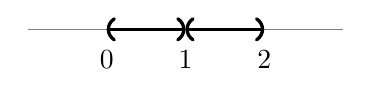
\begin{tikzpicture}
      \draw [help lines] (-1,0) -- (3,0);
      \draw [(-),very thick] (0,0) -- (1,0);
      \draw [(-),very thick] (1,0) -- (2,0);
      \node [below=1ex] at (0,0) {\(0\)};
      \node [below=1ex] at (1,0) {\(1\)};
      \node [below=1ex] at (2,0) {\(2\)};
    \end{tikzpicture}

    \bigskip

    \(X=(0,1)\cup(1,2)\)

    Disjoint/Separated
  \end{minipage}
  \begin{minipage}{3in}
    \centering

    \bigskip

    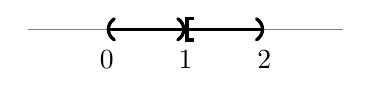
\begin{tikzpicture}
      \draw [help lines] (-1,0) -- (3,0);
      \draw [(-),very thick] (0,0) -- (1,0);
      \draw [[-),very thick] (1,0) -- (2,0);
      \node [below=1ex] at (0,0) {\(0\)};
      \node [below=1ex] at (1,0) {\(1\)};
      \node [below=1ex] at (2,0) {\(2\)};
    \end{tikzpicture}

    \bigskip

    \(X=(0,1)\cup[1,2)\)

    Disjoint/Not Separated
  \end{minipage}
\end{example}

\begin{notation}
  \(X=A|B\) means that \(X=A\cup B\) and \(A\) and \(B\) are separated sets.
\end{notation}

\begin{definition}[Reachable]
  Let \(X\) be a topological space and let \(p,q\in X\).  To say that \(q\) is reachable from \(p\) means that
  for every open cover \(\set{U_{\a}:\a\in\l}\) of \(X\), there exists a finite subset
  \(\set{U_{\a_1},\ldots,U_{\a_n}}\) such that \(p\in U_{\a_1}\), \(q\in U_{\a_n}\), and for all \(1\le k<n\),
  \(U_{\a_k}\cap U_{\a_{k+1}}\ne\emptyset\).
\end{definition}

\begin{lemma}
  Reachable is an equivalence relation.
\end{lemma}

\begin{proof}
  Assume that \(X\) is a topological space, \(\set{U_{\a}:\a\in\l}\) is an open cover for \(X\), and
  \(x,y,z\in X\).
  \begin{description}
  \item[R:] There exists some \(U_{a_k}\) such that \(x\in U_{\a_k}\).  Thus \(x\) is trivially reachable from
    \(x\).

  \item[S:] Assume that \(x\) is reachable from \(y\).  This means that there exists a finite subset
    \(\set{U_{\a_1},\ldots,U_{\a_n}}\) that links \(x\) and \(y\).  Taking those sets in reverse order links
    \(y\) and \(x\).  Therefore \(y\) is reachable from \(x\).

  \item[T:] Assume that \(y\) is reachable from \(x\) and \(z\) is reachable from \(y\).  Then there exists
    a finite subset \(\set{U_{\a_1},\ldots,U_{\a_n}}\) linking \(x\) and \(y\) and a finite subset
    \(\set{U_{\b_1},\ldots,U_{\b_m}}\) linking \(y\) and \(z\).  Let \(U_{\a_j}=U_{\b_k}\) be the first common
    subset in the two paths.  Then \(\set{U_{\a_1},\ldots,U_{\a_j},U_{\b_{k+1}},\ldots,U_{\b_m}}\) is a finite
    subset linking \(x\) and \(z\).  Therefore \(z\) is reachable from \(x\).
  \end{description}
\end{proof}

\begin{theorem}
  Let \(X\) be a topological space.  TFAE:
  \begin{enumerate}
  \item \(X\) is connected.
  \item There are no continuous functions \(f:X\to\R\) such that \(f(X)=\set{0,1}\).
  \item \(X\) is not the union of two disjoint non-empty separated sets.
  \item \(X\) is not the union of two disjoint non-empty closed sets.
  \item The only clopen sets of \(X\) are \(\emptyset\) and \(X\).
  \item For all \(p,q\in X\), \(q\) is reachable from \(p\).
  \end{enumerate}
\end{theorem}

\begin{proof}
  \begin{description}
  \item[]
  \item[\((1\implies2)\)] Assume that \(X\) is connected.

    ABC that there exists a continuous function \(f:X\to\R\) such that \(f(X)=\set{0,1}\).  Let
    \(U=f^{-1}(\set{0})\) and \(V=f^{-1}(\set{1})\).  Since \(\set{0}\) and \(\set{1}\) are closed in \(\R\) and
    \(f\) is continuous, \(U\) and \(V\) are closed in \(X\).  But \(U\sqcup V=X\), so \(U=X-V\) and \(V=X-U\)
    meaning that \(U,V\in\T\) also, contradicting the connectedness of \(X\).

    Therefore there are no continuous functions \(f:X\to\R\) such that \(f(X)=\set{0,1}\).

  \item[\((2\implies3)\)] Assume that there are no continuous functions \(f:X\to\R\) such that \(f(X)=\set{0,1}\).

    ABC that there exists \(A,B\subset X\) such that \(X=A|B\) and consider \(f:X\to\R\) defined by:
    \[f(x)=\begin{cases}
    0, & x\in A \\
    1, & x\in B
    \end{cases}\]
    Now, \(\set{0}\) is closed in \(\R\) and \(f^{-1}(\set{0})=A\).  But \(X=A|B\) and \(\bar{A}\cap B=\emptyset\),
    so \(A\) must contain all of its own limit points, hence \(A=\bar{A}\), meaning that \(A\) is closed in \(X\).
    Similarly, \(B\) is closed in \(X\).  Thus, \(f\) is continuous, contradicting the assumption of non-existence.

    Therefore \(X\) is not the union of two disjoint non-empty separated sets.

  \item[\((3\implies4)\)] (CP) Assume that \(X\) is the union of two disjoint non-empty closed sets.

    This means that there exists \(A\) and \(B\) that are closed in \(X\) such that \(X=A\sqcup B\) and
    \(A,B\ne\emptyset\).  But \(A=\bar{A}\) and so \(\bar{A}\cap B=\emptyset\).  Similarly,
    \(A\cap\bar{B}=\emptyset\).  Thus, \(X=A|B\).

    Therefore \(X\) is the union of two disjoint non-empty separated sets.

  \item[\((4\implies5)\)] (CP) Assume that there exists \(A\) clopen in \(X\) such that \(A\ne\emptyset\) and
    \(A\ne X\).

    This means that \(X-A\) is also clopen.  So \(A\) and \(X-A\) are closed in \(X\), \(X\sqcup(X-A)=X\),
    and \(X,X-A\ne\emptyset\).

    Therefore \(X\) is the union of two disjoint non-empty closed sets.

  \item[\((5\implies6)\)] Assume that the only clopen sets of \(X\) are \(\emptyset\) and \(X\).

    Assume that \(p\in X\) and define \(U=\setb{q\in X}{q\ \text{is reachable from}\ p}\).

    WTS: \(U=X\)

    First, note that \(p\in U\) and so \(U\ne\emptyset\).

    Claim: \(U\in\T\)

    Assume that \(q\in U\).  This means that for any open cover \(\set{U_{\a}:\a\in\l}\) of \(X\) there exists some
    finite subset \(\set{U_{\a_1},\ldots,U_{\a_n}}\) linking \(p\) and \(q\) such that \(q\in U_{\a_n}\).  But
    every other point in \(U_{\a_n}\) is reachable from \(p\), and so \(U_{\a_n}\subset U\).  Thus all \(q\in U\)
    are interior points and therefore \(U\) is open.

    Claim: \(U\) is closed in \(X\)

    Assume that \(q\in\bar{U}\).  This means that for all \(U_q\in\T\) such that \(q\in U_q\), it must be the case
    that \(U_q\cap U\ne\emptyset\).  So any open cover of \(X\) must include some such \(U_q\).  Let
    \(r\in U_q\cap U\).  The \(r\) is reachable from \(p\) and \(r\) is trivially reachable from \(q\), and so
    \(q\) is reachable from \(p\).  Therefore \(q\in U\) and so \(U=\bar{U}\), hence \(U\) is closed.

    Thus \(U\) is clopen and \(U\ne\emptyset\), so \(U=X\).

    Therefore, for all \(p,q\in X\), \(q\) is reachable from \(p\).

  \item[\((6\implies1)\)] Assume that for all \(p,q\in X\), \(q\) is reachable from \(p\).

    ABC that \(X\) is not connected.  This means that there exists \(U,V\in\T\) such that \(U\sqcup V=X\), and so
    \(\set{U,V}\) is an open cover for \(X\).  Now, assume that \(p\in U\) and \(q\in V\).  There is no finite
    subset of this two-set cover that allows \(q\) to be reachable from \(p\), contradicting the assumption.

    Therefore \(X\) is connected.
  \end{description}
\end{proof}

\begin{example}
  Determine whether the following topological spaces are connected or disconnected:
  \begin{enumerate}
  \item \(\R\) with the discrete topology.

    Let \(U=(-\infty,0)\) and \(V=[0,\infty)\).  \(U,V\in\T\) and \(U\sqcup V=\R\).

    Disconnected

  \item \(\R\) with the indiscrete topology.

    \(\T=\set{\emptyset,\R}\), so there are no open non-empty \(U,V\in\T\) such that \(U\sqcup V=\R\).

    Connected

  \item \(\R\) with the cofinite topology.

    ABC there exists non-empty \(U,V\in\T\) such that \(U\sqcup V=\R\).  The \(V=\R-U\) is finite and
    \(U=\R-V\) is finite, meaning that \(U\sqcup V=\R\) is finite, a contradiction.

    Connected.

  \item \(\R_{\text{LL}}\)

    Let \(U=(-\infty,0)\) and \(V=[0,\infty)\).  \(U,V\in\T\) and \(U\sqcup V=\R\).

    Disconnected

  \item \(\Q\) as a subspace of \(R\)

    Let \(U=(-\infty,\pi)\cap\Q\) and \(V=(\pi,\infty)\cap\Q\).  \(U,V\in\T_{\Q}\) and \(U\sqcup V=\Q\).

    Disconnected

  \item \(\R-\Q\) as a subspace of \(R\)

    Let \(U=(-\infty,0)\cap(\R-\Q)\) and \(V=(0,\infty)\cap(\R-\Q)\).  \(U,V\in\T_{\R-\Q}\) and \(U\sqcup V=\R-\Q\).

    Disconnected
  \end{enumerate}
\end{example}

\begin{theorem}
  \(\R_{\text{std}}\) is connected.
\end{theorem}

\begin{proof}
  Since \(\R\) is homeomorphic to \((0,1)\), it is sufficient to show that \((0,1)\) is connected.  So ABC that
  \((0,1)\) is disconnected.  This means that there exists \(A\subset(0,1)\) such that \(A\ne\emptyset,(0,1)\) and
  \(A\) is clopen.  Since \(A\) is bounded, it has a \(\sup\), so let \(a=\sup A\).  But \(A\) is closed, so
  \(a\in A\).  But \(A\) is also open, so there exists \(\e>0\) such that \(B(a,\e)\subset A\), violating the fact
  that \(a=\sup A\).  Therefore \((0,1)\) is connected, and so \(\R\) is connected.
\end{proof}

\begin{corollary}
  An open interval in \(R\) is connected.
\end{corollary}

\begin{definition}[Interval]
  To say that \(I\subset\R\) is an \emph{interval} means that for all \(a,b\in I\), \([a,b]\subset I\).
\end{definition}

\begin{theorem}
  \(C\subset\R\) is connected iff \(C\) is an interval.
\end{theorem}

\begin{proof}
  Assume \(C\subset\R\).
  \begin{description}
  \item[\(\implies\)] Assume that \(C\) is connected.

    ABC that \(C\) is not an interval.  So there exists \(a,b\in C\) such that \([a,b]\not\subset C\).  So there
    exists \(z\in[a,b]\) such that \(z\notin C\).  Let \(U=(-\infty,z)\cap C\) and \(V=(z,\infty)\cap C\).
    \(U,V\in\T_C\), \(U,V\ne\emptyset,C\), and \(U\sqcup V=C\).  Thus, \(C\) is disconnected, contradicting the
    assumption that \(C\) is connected.  Therefore \(C\) is an interval.

  \item[\(\impliedby\)] Assume that \(C\) is an interval.

    Already proved by previous theorem.
  \end{description}
\end{proof}

Note that the union of connected sets need not be connected.  For example, \(U=(0,1)\) and \(V=(1,2)\) are
both connected; however, \(U\sqcup V\) is not an interval and hence is not connected.

\begin{theorem}
  Let \(X\) be a topological space and let \(A,B\subset X\) be separated.  If \(C\subset A\cap B\) is connected
  then either \(C\subset A\) or \(C\subset B\) (but not both).
\end{theorem}

\begin{theorem}
  Let \(X\) be a topological space and let \(\set{C_{\a}:\a\in\l}\) be a collection of connected subsets of \(X\).
  Furthermore, let \(E\subset X\) also be connected such that for all \(\a\in\l\), \(C_{\a}\cap E\ne\emptyset\).
  \(E\cup\bigcup_{\a\in\l}U_{\a}\) is connected.
\end{theorem}

\begin{theorem}
  Let \(X\) be a topological space and let \(C\subset X\) be connected.  If \(D\subset X\) such that
  \(C\subset D\subset\bar{C}\) then \(D\) is connected.
\end{theorem}

\begin{proof}
  Assume \(D\subset X\) such that \(C\subset D\subset\bar{C}\) and ABC that \(D\) is disconnected.  This means that
  there exists \(A,B\subset D\) such that \(A,B\ne\emptyset\) and \(D=A|B\).  Now, since \(C\subset D\), it must be
  the case that either \(C\subset A\) or \(C\subset B\) (but not both).  So AWLOG that \(C\subset A\), and hence
  \(\bar{C}\subset\bar{A}\).  But \(\bar{A}\cap B=\emptyset\) and so \(\bar{C}\cap B=\emptyset\).  And since
  \(D\subset\bar{C}\), \(D\subset B=\emptyset\).  But this can only be the case if \(B=\emptyset\), contradicting
  the assumption that \(B\) is not empty.  Therefore \(D\) is connected.
\end{proof}

\begin{corollary}
  Let \(X\) be a topological space and \(C\subset X\).  If \(C\) is connected then \(\bar{C}\) is connected.
\end{corollary}

\begin{proof}
  Assume that \(C\) is connected.  But \(C\subset\bar{C}\subset\bar{C}\).  Therefore, by previous theorem,
  \(\bar{C}\) is connected.
\end{proof}

\begin{theorem}
  The closure of the topologist's sine curve in \(\R^2\) is connected.
\end{theorem}

\begin{proof}
  Let:
  \begin{gather*}
    S=\setb{\left(x,\sin\left(\frac{1}{x}\right)\right)}{x\in(0,1)} \\
    \\
    \bar{S}=S\cup\set{(1,\sin(1))}\cup\setb{(0,y)}{y\in[-1,1]}
  \end{gather*}
  ABC that \(S\) is not connected.  This means that there exists \(g:S\to\set{0,1}\) such that \(g\) is continuous
  and surjective.  But \(f:(0,1)\to S\) defined by \(f(x)=(x,\sin\frac{1}{x})\) is also continuous and surjective.
  This means that \(g\circ f:(0,1)\to\set{0,1}\) is also continuous and surjective, indicating that \((0,1)\)
  is not connected, contradicting the connectedness of the interval.  Therefore \(S\) is connected, and by
  previous corollary, \(\bar{S}\) is connected.
\end{proof}

\begin{theorem}
  Let \(X\) and \(Y\) be a topological spaces and let \(f:X\to Y\) be continuous and surjective.  If \(X\) is
  connected then \(Y\) is connected.
\end{theorem}

\begin{proof}
  Assume that \(X\) is connected and ABC that \(Y\) is disconnected.  This means that there exists \(U,V\in\T_Y\)
  such that \(U,V\ne\emptyset\) and \(U\sqcup V=Y\).  Now, since \(f\) is continuous, \(f^{-1}(U),f^{-1}(V)\in\T_X\).
  Furthermore, since \(f\) is surjective, \(f^{-1}(U),f^{-1}(V)\ne\emptyset\) and \(f^{-1}(U)\sqcup f^{-1}(V)=X\).
  Thus, \(X\) is disconnected, violating the assumption.  Therefore \(Y\) is connected.
\end{proof}

\begin{corollary}
  Let \(X\) and \(Y\) be homemorphic topological spaces.  \(X\) is connected iff \(Y\) is connected.
\end{corollary}

\begin{proof}
  It is sufficent to prove one direction, so assume that \(X\) is connected.  This means that there exists a
  homeomorphism \(f:X\to Y\).  But homeomorphism are continuous and surjective.  Therefore \(Y\) is connected.
\end{proof}

\begin{theorem}[IVT]
  Let \(f:\R\to\R\) be continuous and \((a,b)\subset\R\).  If \(f(a)<r<f(B)\) then there exists \(c\in(a,b)\)
  such that \(f(c)=r\).
\end{theorem}

\begin{proof}
  Assume that \(f(a)<r<f(b)\).  Since \([a,b]\) is connected and \(f\) is continuous, \(f([a,b])\) is connected,
  and hence \(f([a,b])\) must be an interval.  But \(f(a),f(b)\in f([a,b])\) and \(f(a)<r<f(b)\), so \(r\in
  f((a,b))\).  Therefore, there must exist some \(c\in(a,b)\) such that \(f(c)=r\).
\end{proof}

\begin{theorem}
  Let \(X\) and \(Y\) be topological spaces.  \(X\times Y\) is connected iff \(X\) and \(Y\) are connected.
\end{theorem}

\begin{proof}
  \begin{description}
  \item[]
  \item[\(\implies\)] Assume that \(X\times Y\) is connected.

    \(\pi_X\) and \(\pi_Y\) are continuous and surjective.  Therefore \(X\) and \(Y\) are connected.

  \item[\(\impliedby\)] Assume that \(X\) and \(Y\) are connected.

    Assume \(x_0\in X\) and consider \(\set{x_0}\times Y\).  Since \(\set{x_0}\times Y\) is homeomorphic to \(Y\) and
    \(Y\) is connected, \(\set{x_0}\times Y\) is connected.  Similarly, for all \(y\in Y\), \(X\times\set{y}\) is
    connected.  Note that \(X\times Y=\bigcup_{y\in Y}X\times\set{y}\).  Furthermore, for all \(y\in Y\):
    \[(\set{x_0}\times Y)\cap(X\times\set{y})=\set{(x_0,y)}\ne\emptyset\]
    Therefore, by previous theorem, \(X\times Y\) is connected.
  \end{description}
\end{proof}

\end{document}
